% This is a Basic Assignment Paper but with like Code and stuff allowed in it, there is also url, hyperlinks from contents included. 

\documentclass[11pt]{article}

% Preamble

\usepackage[margin=1in]{geometry}
\usepackage{amsfonts, amsmath, amssymb}
\usepackage{fancyhdr, float, graphicx}
\usepackage[utf8]{inputenc} % Required for inputting international characters
\usepackage[T1]{fontenc} % Output font encoding for international characters
\usepackage{fouriernc} % Use the New Century Schoolbook font
\usepackage[nottoc, notlot, notlof]{tocbibind}
\usepackage{listings}
\usepackage{xcolor}
\usepackage{blindtext}
\usepackage{hyperref}
\hypersetup{
    colorlinks=true,
    linkcolor=black,
    filecolor=magenta,      
    urlcolor=cyan,
    pdfpagemode=FullScreen,
    }

\definecolor{codegreen}{rgb}{0,0.6,0}
\definecolor{codegray}{rgb}{0.5,0.5,0.5}
\definecolor{codepurple}{rgb}{0.58,0,0.82}
\definecolor{backcolour}{rgb}{0.95,0.95,0.92}

\lstdefinestyle{mystyle}{
    backgroundcolor=\color{backcolour},   
    commentstyle=\color{codegreen},
    keywordstyle=\color{magenta},
    numberstyle=\tiny\color{codegray},
    stringstyle=\color{codepurple},
    basicstyle=\ttfamily\footnotesize,
    breakatwhitespace=false,         
    breaklines=true,                 
    captionpos=b,                    
    keepspaces=true,                 
    numbers=left,                    
    numbersep=5pt,                  
    showspaces=false,                
    showstringspaces=false,
    showtabs=false,                  
    tabsize=2
}

\lstset{style=mystyle}

% Header and Footer
\pagestyle{fancy}
\fancyhead{}
\fancyfoot{}
\fancyhead[L]{\textit{\Large{Internet of Things Lab Assignment 6}}}
\fancyhead[R]{\textit{\Large{Krishnaraj}}}
%\fancyhead[R]{\textit{something}}
\fancyfoot[C]{\thepage}
\renewcommand{\footrulewidth}{1pt}



% Other Doc Editing
% \parindent 0ex
%\renewcommand{\baselinestretch}{1.5}

\begin{document}

\begin{titlepage}
	\centering

	%---------------------------NAMES-------------------------------

	\huge\textsc{
		MIT World Peace University
	}\\

	\vspace{0.75\baselineskip} % space after Uni Name

	\LARGE{
		Internet of Things\\
		Second Year B. Tech, Semester 2
	}

	\vfill % space after Sub Name

	%--------------------------TITLE-------------------------------

	\rule{\textwidth}{1.6pt}\vspace*{-\baselineskip}\vspace*{2pt}
	\rule{\textwidth}{0.6pt}
	\vspace{0.75\baselineskip} % Whitespace above the title



	\huge{\textsc{
			MQTT Protocol Implementation using Tinkercad on Arduino UNO
		}} \\



	\vspace{0.5\baselineskip} % Whitespace below the title
	\rule{\textwidth}{0.6pt}\vspace*{-\baselineskip}\vspace*{2.8pt}
	\rule{\textwidth}{1.6pt}

	\vspace{1\baselineskip} % Whitespace after the title block

	%--------------------------SUBTITLE --------------------------	

	\LARGE\textsc{
		Assignment 6
	} % Subtitle or further description
	\vfill

	%--------------------------AUTHOR-------------------------------

	Prepared By
	\vspace{0.5\baselineskip} % Whitespace before the editors

	\Large{
		Krishnaraj Thadesar \\
		Cyber Security and Forensics\\
		Batch A2, PA 20
	}


	\vspace{0.5\baselineskip} % Whitespace below the editor list
	\today

\end{titlepage}


\tableofcontents
\thispagestyle{empty}
\clearpage

\setcounter{page}{1}

\section{Aim}

To understand the working of MQTT Protocol and implement it using Tinkercad on Arduino UNO.

\section{Objectives}
\begin{enumerate}
	\item To understand the working of MQTT Protocol.
	\item To use Arduino UNO to implement the MQTT Protocol.
	\item To sense data from sensors and send it to cloud.
\end{enumerate}

\section{Equipments Used}

\begin{table}[H]
	\begin{tabular}{|c|c|c|}
		\hline
		\textbf{Name}                                   & \textbf{Quantity} & \textbf{Component}             \\ \hline
		U1                                              & 1                 & Arduino Uno R3                 \\ \hline
		U2                                              & 1                 & Temperature Sensor {[}TMP36{]} \\ \hline
		U3                                              & 1                 & Wifi Module (ESP8266)          \\ \hline
		\begin{tabular}[c]{@{}c@{}}R1\\ R2\end{tabular} & 2                 & 1 kΩ Resistor                  \\ \hline
	\end{tabular}
\end{table}

\section{Theory}
Our project involves sensing the temperature using the TMP36 sensor and sending the data to the cloud using the ESP8266 module and MQTT protocol. This is an example of \textbf{sensing}.

\subsection{MQTT}
MQTT (Message Queuing Telemetry Transport) is a lightweight messaging protocol that is widely used in IoT (Internet of Things) applications for sending and receiving data between devices and the cloud. It uses a publish/subscribe messaging model, where devices (publishers) send messages to a central server (broker), which then distributes the messages to other devices (subscribers) that have subscribed to the topic of the message.

\subsection{Connection}
In our project, we use the ESP8266 module to connect to the Internet and publish the temperature data to a cloud platform called Thingspeak using the MQTT protocol. Thingspeak is a platform that allows users to collect, analyze, and visualize data from IoT devices. It provides an MQTT broker that can be used to publish and subscribe to data streams, as well as a web interface for displaying and analyzing the data in real-time.\\

To use MQTT in our project, we would need to first establish a connection to the broker using the ESP8266 module and then publish the temperature data to a specific topic on the broker. We could then use the Thingspeak API to retrieve the data from the broker and display it in a chart or graph on the Thingspeak web interface.


\section{Circuit Diagram}
\begin{figure}[H]
	\centering
	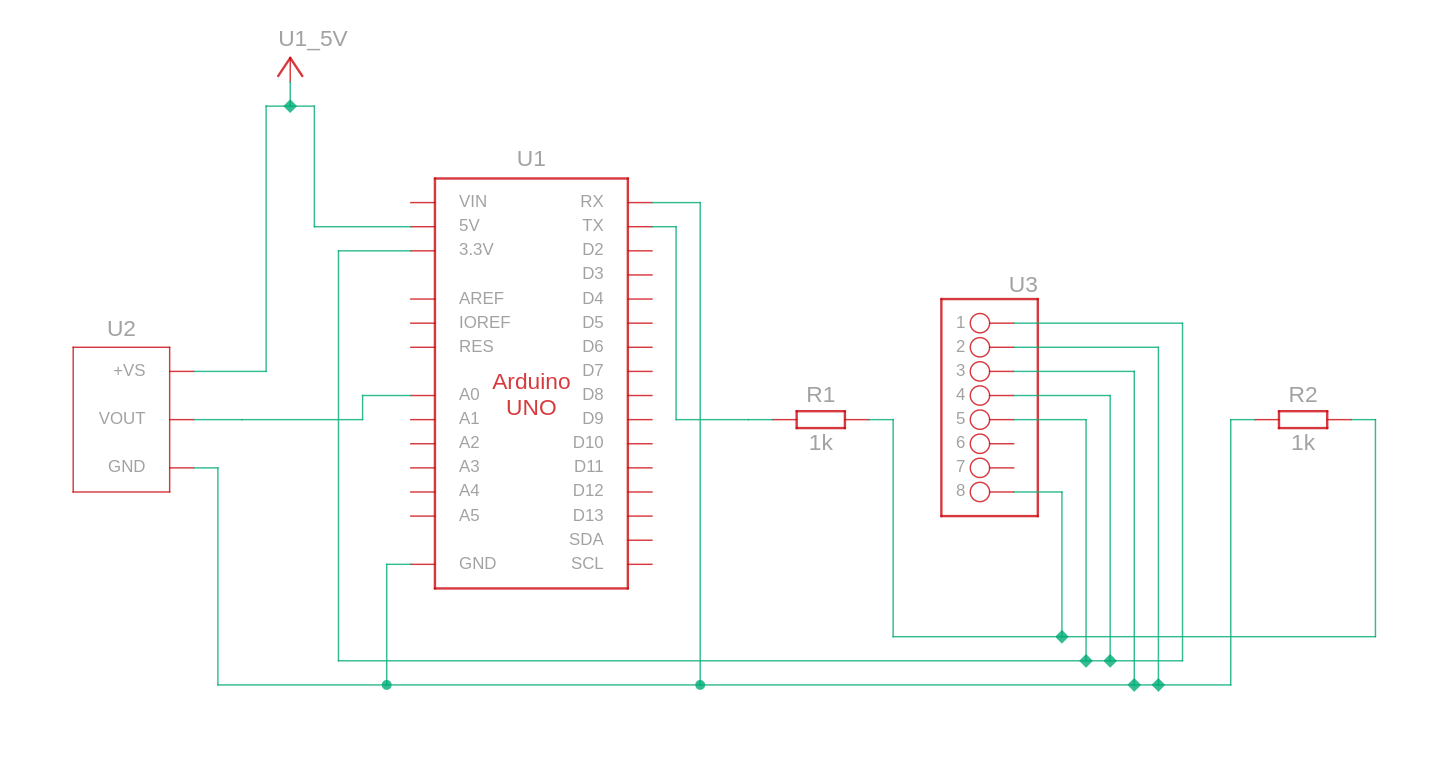
\includegraphics[width=.95\textwidth]{Screenshot_on_2023-05-01_at_15-01-59.png}
	\caption{Circuit Diagram}
\end{figure}

\begin{figure}[H]
	\centering
	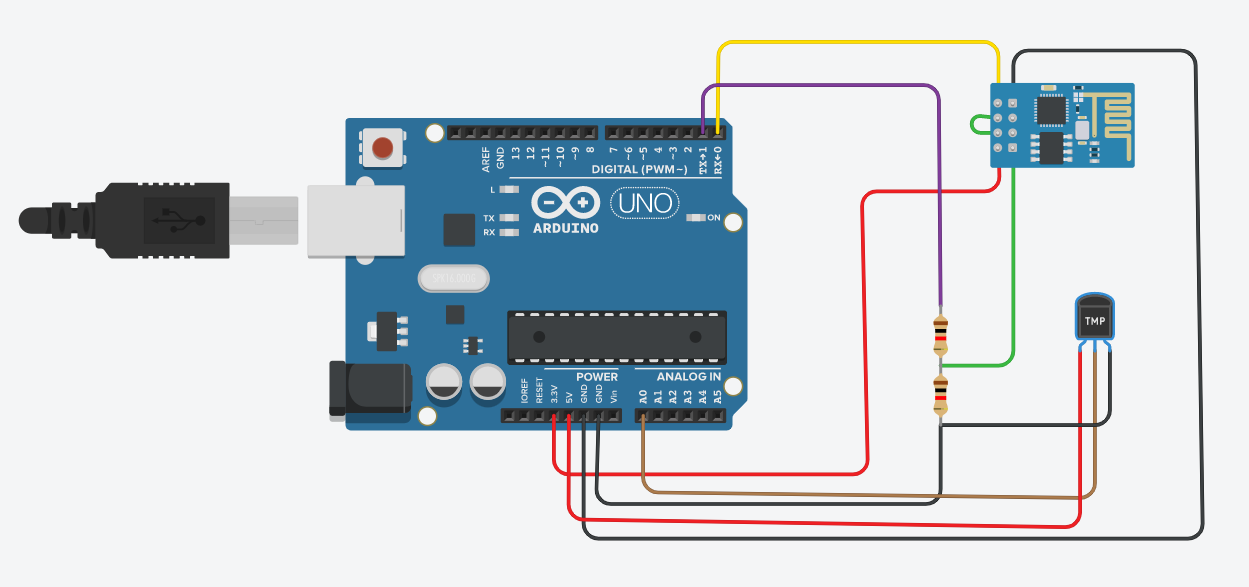
\includegraphics[width=.95\textwidth]{Screenshot_on_2023-05-01_at_15-48-33.png}
	\caption{Circuit}
\end{figure}

\section{Platform}
\textbf{Operating System}: Arch Linux x86-64 \\
\textbf{IDEs or Text Editors Used}: Visual Studio Code and Tinkercad\\
% \textbf{Compilers} : g++ and gcc on linux for C++, and javac, with JDK 18.0.2 for Java\\

\section{Input}
Data from the Temperature Sensor is sent to the cloud using the MQTT Protocol.
\section{Output}
\begin{verbatim}
CIPSEND=89
GET /update?api_key=SGXV2O1YIK6KJ2SC &field1=76.47 HTTP/1.1
Host: api.thingspeak.com

AT+CIPSEND=89
GET /update?api_key=SGXV2O1YIK6KJ2SC &field1=76.47 HTTP/1.1
Host: api.thingspeak.com

AT+CIPSEND=90
GET /update?api_key=SGXV2O1YIK6KJ2SC &field1=199.52 HTTP/1.1
Host: api.thingspeak.com

AT+CIPSEND=90
GET /update?api_key=SGXV2O1YIK6KJ2SC &field1=256.65 HTTP/1.1
Host: api.thingspeak.com

AT+CIPSEND=90
GET /update?api_key=SGXV2O1YIK6KJ2SC &field1=108.99 HTTP/1.1
Host: api.thingspeak.com

AT+CIPSEND=90
GET /update?api_key=SGXV2O1YIK6KJ2SC &field1=-40.42 HTTP/1.1
Host: api.thingspeak.com
\end{verbatim}


\section{Code}
\begin{lstlisting}[language=C++]
float val, voltage, temp,tempf;
String ssid     = "Simulator Wifi";  // SSID to connect to
String password = ""; //virtual wifi has no password 
String host     = "api.thingspeak.com"; // Open Weather Map API
const int httpPort   = 80;
String url     = "/update?api_key=SGXV2O1YIK6KJ2SC";
String url1     = " &field1=";
//Replace XXXXXXXXXXXXXXXX by your ThingSpeak Channel API Key

void setupESP8266(void) {
	
	// Start our ESP8266 Serial Communication
	Serial.begin(115200);   // Serial connection over USB to computer
	Serial.println("AT");   // Serial connection on Tx / Rx port to ESP8266
	delay(10);        // Wait a little for the ESP to respond
	if (Serial.find("OK"))
	Serial.println("ESP8266 OK!!!");
	
	// Connect to Simulator Wifi
	Serial.println("AT+CWJAP=\"" + ssid + "\",\"" + password + "\"");
					
	
	
	delay(10);        // Wait a little for the ESP to respond
	if (Serial.find("OK"))
	Serial.println("Connected to WiFi!!!");
	
	// Open TCP connection to the host:
	//ESP8266 connects to the server as a TCP client. 

	Serial.println("AT+CIPSTART=\"TCP\",\"" + host + "\"," + httpPort);
	delay(50);        // Wait a little for the ESP to respond
	if (Serial.find("OK")) 
	Serial.println("ESP8266 Connected to server!!!") ;
	
}

void anydata(void) {
	
	val=analogRead(A0);
	voltage=val*0.0048828125; 
	temp = (voltage - 0.5) * 100.0;
	tempf=(temp*9/5)+32;
	//distance=12;

	// Construct our HTTP call
	String httpPacket = "GET " + url  + url1 + String(tempf) + " HTTP/1.1\r\nHost: " + host + "\r\n\r\n";
	int length = httpPacket.length();
	
	// Send our message length
	Serial.print("AT+CIPSEND=");
	Serial.println(length);
	delay(10); // Wait a little for the ESP to respond if (!Serial.find(">")) return -1;

	// Send our http request
	Serial.print(httpPacket);
	delay(10); // Wait a little for the ESP to respond
	if (Serial.find("SEND OK\r\n"))
	Serial.println("ESP8266 sends data to the server");
	
}

void setup() {
	pinMode(A0, INPUT);
	setupESP8266();
				
}

void loop() {
	
	anydata();
	
	delay(100);
}
\end{lstlisting}
\section{Conclusion}
Thus, we have successfully sent data from the Temperature Sensor to the cloud using the MQTT Protocol.
\clearpage

\section{FAQ}

Details of the main components used in this project and their pin specifications:

\begin{enumerate}
	\item Arduino Uno R3 (Code: U1)
	      \begin{itemize}
		      \item Type: Microcontroller board
		      \item Digital pins: 14
		      \item Analog input pins: 6
		      \item Operating voltage: 5V
		      \item Input voltage (recommended): 7-12V
		      \item Input voltage (limits): 6-20V
		      \item Flash memory: 32 KB (ATmega328P microcontroller)
		      \item SRAM: 2 KB (ATmega328P microcontroller)
		      \item EEPROM: 1 KB (ATmega328P microcontroller)
		      \item Clock speed: 16 MHz (ATmega328P microcontroller)
	      \end{itemize}
	\item Temperature Sensor [TMP36] (Code: U2)
	      \begin{itemize}
		      \item Type: Analog sensor
		      \item Pin 1: Output voltage (analog)
		      \item Pin 2: Ground
		      \item Pin 3: Input voltage (3.3V - 5V)
		      \item Temperature range: -40°C to +125°C
		      \item Output voltage range: 0V to 1.75V (at 25°C)

	      \end{itemize}
	\item Wifi Module [ESP8266] (Code: U3)
	      \begin{itemize}
		      \item Type: Digital communication module
		      \item Pin 1: VCC (3.3V)
		      \item Pin 2: Ground
		      \item Pin 3: TXD (Transmit Data)
		      \item Pin 4: RXD (Receive Data)
		      \item Operating voltage: 3.3V
		      \item Communication protocol: UART
		      \item Wireless standard: IEEE 802.11 b/g/n
	      \end{itemize}
	\item 1 kΩ Resistor (Codes: R1 and R2)

	      \begin{itemize}
		      \item Type: Resistor
		      \item Resistance: 1 kΩ (1000 ohms)
		      \item Tolerance: 5\%
		      \item Power rating: 1/4 watt
		      \item Quantity: 2
	      \end{itemize}

\end{enumerate}

\end{document}